\documentclass[a4paper,12pt]{article} 

%%% Работа с русским языком
\usepackage{cmap}					% поиск в PDF
\usepackage{mathtext} 				% русские буквы в фомулах
\usepackage[T2A]{fontenc}			% кодировка
\usepackage[utf8]{inputenc}			% кодировка исходного текста
\usepackage[english,russian]{babel}	% локализация и переносы

%%% Дополнительная работа с математикой
\usepackage{amsmath,amsfonts,amssymb,amsthm,mathtools, gensymb} % AMS
\usepackage{icomma} % "Умная" запятая: $0,2$ --- число, $0, 2$ --- перечисление

%%Таблица
\usepackage[table,xcdraw]{xcolor}
\usepackage{caption}
\usepackage{subcaption}
\usepackage{floatrow}
\floatsetup[table]{capposition=top}
\floatsetup[wrapfigure]{capposition=bottom}
%multi-column
%\usepackage{multi-column}
%multi-row
\usepackage{multirow}


%% Номера формул
\mathtoolsset{showonlyrefs=true} % Показывать номера только у тех формул, на которые есть \eqref{} в тексте.

%% Шрифты
\usepackage{euscript}	 % Шрифт Евклид
\usepackage{mathrsfs} % Красивый матшрифт

%% Свои команды
\DeclareMathOperator{\sgn}{\mathop{sgn}}

%% Перенос знаков в формулах (по Львовскому)
\newcommand*{\hm}[1]{#1\nobreak\discretionary{}
{\hbox{$\mathsurround=0pt #1$}}{}}

%% Стиль страницы
\usepackage{fancyhdr}

%% Для рисунков
\usepackage{graphicx}
\usepackage[export]{adjustbox}
\usepackage{float}
\usepackage{ragged2e}
\usepackage{wrapfig}

%Отступы и поля 
\textwidth=20cm
\oddsidemargin=-2cm
\topmargin=-2cm
\textheight=25cm

\pagestyle{fancy}
\begin{document}
\begin{titlepage}
\begin{center}
%\vspace*{1cm}
\large{\small ФЕДЕРАЛЬНОЕ ГОСУДАРСТВЕННОЕ АВТОНОМНОЕ ОБРАЗОВАТЕЛЬНОЕ\\ УЧРЕЖДЕНИЕ ВЫСШЕГО ОБРАЗОВАНИЯ \\ МОСКОВСКИЙ ФИЗИКО-ТЕХНИЧЕСКИЙ ИНСТИТУТ\\ (НАЦИОНАЛЬНЫЙ ИССЛЕДОВАТЕЛЬСКИЙ УНИВЕРСИТЕТ)\\ ФАКУЛЬТЕТ АЭРОКОСМИЧЕСКИХ ТЕХНОЛОГИЙ}
\vfill
\line(1,0){430}\\[1mm]
%\huge{Лабораторная 2}\\
\huge\textbf{Расчёт статически определимой фермы}\\
\line(1,0){430}\\[1mm]
\vfill
\begin{flushright}
\normalsize{Рогозин Владимир}\\
\normalsize{\textbf{Группа Б03-106}}\\
\end{flushright}
\end{center}
\end{titlepage}
\fancyhead[c] {Расчёт статически определимой фермы}

\textbf{Цель работы:} 
Ознакомление и расчёт сил в стержнях статически определённой фермы.

\textbf{Теоретические сведения:} \textit{Стержень} -- элемент конструкции, представляющий собой удлинённое тело. Мтержневая система состоит из \textit{стержней, узлов и опор}. \textit{Узел} -- место соединения стержней. Если углы могут меняться свободно, такой узел называется \textit{шарниром}. Если перемещения узлов возможны только за счёт деформации стержней, то такая стержневая система называется \textit{геометрически неизменяемой}.

Существуют следующие геометрически неизменяемые стержневые системы: 
\textit{рамы, фермы} и системы \textit{смешанного типа}, имеющие в своём составе элементы первых двух видов. \textit{Механизм} -- система, которая может совершать движение около неподвижных точек без деформации элементов. Если при замене жестких соединений стержней в системе на шарниры она превращается в механизм, то это рама, иначе -- ферма. 

На стержневую систему могут действовать сосредоточенные и распределённые силы, а также сосредоточенные и распределённые моменты. Если узлы стержневой системы и действующие на неё нагрузки лежат в одной плоскости, то такая система назвается \textit{плоской}. В противном случае система называется \textit{пространственной}.

Далее будем рассматривать плоские фермы, на которые действуют сосредоточенные силы, приложенные только к углам. Если силы приложены таким образом, то в стержнях отсутствуют изгибающие моменты, то есть стержни работают только на сжатие и растяжение.

Числом \textit{степеней свободы} называется количество независимых параметров, которыми можно описать взаимное расположение элементов в системе. Ограничение свободных перемещений элементов системы называется \textit{связями}. Количество связей в соединении равно количеству устраняемых ими возможных перемещений.

Количество степеней свободы $N$ фермы можно вычислить по формуле
\[N = 2N_{node} - N_{rod} - N_0\]
где $N_{node}$ -- количество узлов, $N_{rod}$ -- количество стержней, $N_0$ -- количество связей, накладываемых опорами.

Будем рассматривать опоры ферм следующих видов: \par
1) шарнирно-подвижная опора \par
2) шарнирно-неподвижная опора \par
Шарнирно-подвижная опора позволяет опорному узлу двигаться в одном направлении, запрещая перемещаться в перпендикулярном, то есть накладывает 1 связь. Шарнирно-неподвижная опора в принципе запрещает опорному узлу перемещаться, то есть накладывает 2 связи.

\textit{Статически определимой} системой называется система, для которой силы в стержнях можно определить только из уравнений статики. 

\textit{Статически неопределимой} системой называется система, для которой уравнений равновесия недостаточно и требуются дополнительные соотношения, такие как уравнение совместности деформаций.

Количество уравнений статики для системы узлов равно $2N_{node}$, а количество неизвестных сил в стержнях и опорах равно количеству стержней и количеству связей, накладываемых опорами. Таким образом, условие статической определимости фермы можно записать в виде
\[N = 0\]
Если 
\[N < 0\text{,}\]
то система статически неопределима.


\textbf{Расчёт статически определимой фермы}\\
\textbf{Способ вырезания узлов.} В \textit{способе вырезания узлов} рассматривается равновесие отдельно взятого узла. В шарнире момент сил равен нулю и линии действия всех сил, относящихся к узлу, пересекаются в одной точке, не создавая моментов. Таким образом, для каждого угла можно составить только два уравнения равновесия. Способ вырезания узлом удобен, если в каждом узле, для которого составляются условия равновесия, сходятся один стержень с известной силой и два с неизвестной. Начинается расчёт с узла, где сходятся два стержня.

Рассмотренный метод удобен для ручных вычислений, но для численных расчетов на ЭВМ не применяется из-за быстрого накопления ошибок.

\textbf{Способ моментной точки.} Иногда нужно вычислить усилия только в определенном стержне. Для этого применяется другой способ -- \textit{способ моментной точки}. В этом способе смотрятся моменты сил относительно определённой точки, выбранной таким образом, чтобы моменты неизвестных сил, приложенных к точке, занулились, а момент  искомой силы был равен моментам других, уже известных.   

\textbf{Матричная форма вычисления сил.} Для расчёта статически определимых ферм способом вырезания узлом на ЭВМ систему уравнений равновесия для всех узлов можно представить в матричном виде. Уравнения равновесия $k$-го узла имеют вид
\[\sum_i N_i \cos \alpha_{ik} + F_{kx} = 0\]
\[\sum_i N_i \sin \alpha_{ik} + F_{ky} = 0\]
где $\alpha_{ik}$ -- угол между положительным направлениями силы $N_i$ в $i$-ом стержне и оси $x$ в $k$-ом узле.

В матричном виде система уравнений имеет вид
\[\mathbf{CN + F} = 0 \text{,}\]
где 
\begin{equation}
    \begin{aligned}
        \mathbf{N} = \begin{vmatrix}
            N_1 \\
            N_2 \\ 
            ... \\
            N_n
        \end{vmatrix} \text{,}\quad & 
        \mathbf{F} = \begin{vmatrix}
                F_{1x} \\
                F_{1y} \\
                F_{2x} \\
                F_{2y} \\ 
                ... \\
                F_{mx} \\
                F_{my}
            \end{vmatrix}
    \end{aligned}
\end{equation}

В число нагрузок $N$ включены также силы реакции опоры. Ферма статически определима, следовательно 
\[n = 2m\]

Матрица $C$ имеет размерность $n \times n$ и содержит $\cos \alpha_{ik}$ и $\sin \alpha_{ik}$ и нули для тех стержней, которые не примыкают к $k$-ому узлу.

Вычисление нагрузок сводится к высилению обратной матрицы $\mathbf{C}^{-1}$. Для геометрически неизменяемых стрежневых систем det$\mathbf{C} \neq 0$  и решение всегда существует
\[\mathbf{N} = -\mathbf{C}^{-1}\mathbf{F}\]

\textbf{Расчёт статически неопределимой фермы}\\
 Для расчета сил в стержнях в статически неопределимых фермах уравнений статики недостаточно, нужны дополнительные соотношения, выражающие условия совместности деформаций.

 Для получения дополнительных соотношений можно использовать теорему Кастильяно, которая формулируется следующим образом:
\[y_i = \frac{\partial W}{\partial P_i} \text{,}\]
где $y_i$ -- перемещение вдоль линии действия силы $P_i$, $W$ -- полная упругая энергия системы.

\textbf{Обработка данных:} 
\begin{figure}[H]\label{fig: Ustanovka}
    \centering
    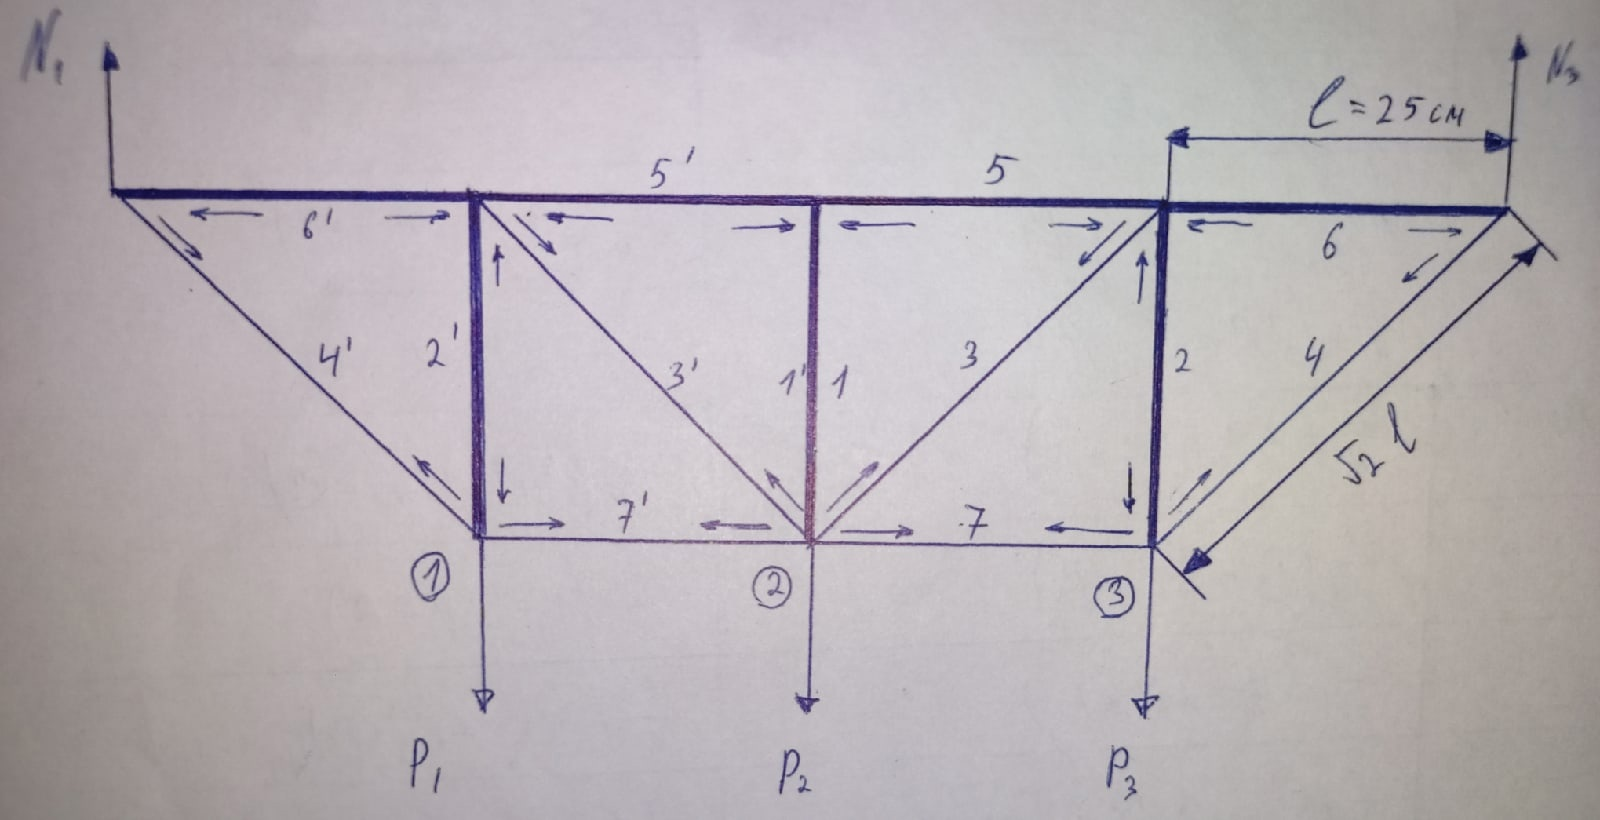
\includegraphics[width = \textwidth]{Ферма.png}
    \caption{Для расчёта сил в стержнях в произвольном случае}
\end{figure}

Параметры системы: $d_2 = 10$ мм -- внешний диаметр полого стержня,  $d_1 = 4$ мм -- внутренний диаметр полого стержня, $d = 4,2$ мм -- диаметр сплошного стержня, $l = 25$ см -- длина вертикальных и горизонтальных стержней, $\sqrt{2} l \approx 35,36$ см -- длина косых стержней. Модуль Юнга материала, из которого сделаны стержни, равен $E = 2 \cdot 10^{6}$ $кг/cм^2$. Стержни под номерами 1, 2, 5, 6 полые, под номерами 3, 4, 7 (и соответствующие им штрихованные) -- сплошные.

В данной установке стержни 5, 5', 6 и 6' сдвоенные.

В работе система нагружалась двумя различными способами, а именно: \\
I) $P_1 = P_3 = 0$, $P_2 = 100$ Н \\
II) $P_1 = P_2 = P_3 = 100$ Н \\
В таблице ниже приведены результаты теоретической оценки и экспериментальных данных для обоих случаев. 

\begin{table}[H]\label{tab: Power Datchiks}
    \centering
    \begin{tabular}{|
        >{\columncolor[HTML]{FFFFFF}}c 
        >{\columncolor[HTML]{FFFFFF}}c 
        >{\columncolor[HTML]{FFFFFF}}c |
        >{\columncolor[HTML]{FFFFFF}}c 
        >{\columncolor[HTML]{FFFFFF}}c 
        >{\columncolor[HTML]{FFFFFF}}c |}
        \hline
        \multicolumn{3}{|c|}{\cellcolor[HTML]{FFFFFF}{\color[HTML]{000000} I}} &
          \multicolumn{3}{c|}{\cellcolor[HTML]{FFFFFF}{\color[HTML]{000000} II}} \\ \hline
        \multicolumn{1}{|c|}{\cellcolor[HTML]{FFFFFF}{\color[HTML]{000000} $N$}} &
          \multicolumn{1}{c|}{\cellcolor[HTML]{FFFFFF}{\color[HTML]{000000} $F_{теор}$, H}} &
          {\color[HTML]{000000} $F_{эксп}$, H} &
          \multicolumn{1}{c|}{\cellcolor[HTML]{FFFFFF}{\color[HTML]{000000} $N$}} &
          \multicolumn{1}{c|}{\cellcolor[HTML]{FFFFFF}{\color[HTML]{000000} $F_{теор}$, H}} &
          {\color[HTML]{000000} $F_{эксп}$, H} \\ \hline
        \multicolumn{1}{|c|}{\cellcolor[HTML]{FFFFFF}{\color[HTML]{000000} 1}} &
          \multicolumn{1}{c|}{\cellcolor[HTML]{FFFFFF}{\color[HTML]{000000} 0}} &
          {\color[HTML]{000000} 0,3} &
          \multicolumn{1}{c|}{\cellcolor[HTML]{FFFFFF}{\color[HTML]{000000} 1}} &
          \multicolumn{1}{c|}{\cellcolor[HTML]{FFFFFF}{\color[HTML]{000000} 0}} &
          {\color[HTML]{000000} 0,8} \\ \hline
        \multicolumn{1}{|c|}{\cellcolor[HTML]{FFFFFF}{\color[HTML]{000000} 2}} &
          \multicolumn{1}{c|}{\cellcolor[HTML]{FFFFFF}{\color[HTML]{000000} $P / 2$ = 50,0}} &
          {\color[HTML]{000000} 51,0} &
          \multicolumn{1}{c|}{\cellcolor[HTML]{FFFFFF}{\color[HTML]{000000} 2}} &
          \multicolumn{1}{c|}{\cellcolor[HTML]{FFFFFF}{\color[HTML]{000000} $P / 2$ = 50,0}} &
          {\color[HTML]{000000} 50,2} \\ \hline
        \multicolumn{1}{|c|}{\cellcolor[HTML]{FFFFFF}{\color[HTML]{000000} 3}} &
          \multicolumn{1}{c|}{\cellcolor[HTML]{FFFFFF}{\color[HTML]{000000} $\sqrt{2}P / 2$ = 70,7}} &
          {\color[HTML]{000000} 71,6} &
          \multicolumn{1}{c|}{\cellcolor[HTML]{FFFFFF}{\color[HTML]{000000} 3}} &
          \multicolumn{1}{c|}{\cellcolor[HTML]{FFFFFF}{\color[HTML]{000000} $\sqrt{2}P / 2$ = 70,7}} &
          {\color[HTML]{000000} 70,6} \\ \hline
        \multicolumn{1}{|c|}{\cellcolor[HTML]{FFFFFF}{\color[HTML]{000000} 4}} &
          \multicolumn{1}{c|}{\cellcolor[HTML]{FFFFFF}{\color[HTML]{000000} $\sqrt{2}P / 2$ = 70,7}} &
          {\color[HTML]{000000} 70,7} &
          \multicolumn{1}{c|}{\cellcolor[HTML]{FFFFFF}{\color[HTML]{000000} 4}} &
          \multicolumn{1}{c|}{\cellcolor[HTML]{FFFFFF}{\color[HTML]{000000} $3\sqrt{2}P / 2$ = 212,1}} &
          {\color[HTML]{000000} 212,7} \\ \hline
        \multicolumn{1}{|c|}{\cellcolor[HTML]{FFFFFF}{\color[HTML]{000000} 5}} &
          \multicolumn{1}{c|}{\cellcolor[HTML]{FFFFFF}{\color[HTML]{000000} $P / 2$ = 50,0}} &
          {\color[HTML]{000000} 58,8} &
          \multicolumn{1}{c|}{\cellcolor[HTML]{FFFFFF}{\color[HTML]{000000} 5}} &
          \multicolumn{1}{c|}{\cellcolor[HTML]{FFFFFF}{\color[HTML]{000000} $P$ = 100}} &
          {\color[HTML]{000000} 119,0} \\ \hline
        \multicolumn{1}{|c|}{\cellcolor[HTML]{FFFFFF}{\color[HTML]{000000} 6}} &
          \multicolumn{1}{c|}{\cellcolor[HTML]{FFFFFF}{\color[HTML]{000000} $P / 2$ = 50,0}} &
          {\color[HTML]{000000} 25,9} &
          \multicolumn{1}{c|}{\cellcolor[HTML]{FFFFFF}{\color[HTML]{000000} 6}} &
          \multicolumn{1}{c|}{\cellcolor[HTML]{FFFFFF}{\color[HTML]{000000} $3P / 4$ = 75,0}} &
          {\color[HTML]{000000} 79,3} \\ \hline
        \multicolumn{1}{|c|}{\cellcolor[HTML]{FFFFFF}{\color[HTML]{000000} 7}} &
          \multicolumn{1}{c|}{\cellcolor[HTML]{FFFFFF}{\color[HTML]{000000} $P / 2$ = 50,0}} &
          {\color[HTML]{000000} 51,4} &
          \multicolumn{1}{c|}{\cellcolor[HTML]{FFFFFF}{\color[HTML]{000000} 7}} &
          \multicolumn{1}{c|}{\cellcolor[HTML]{FFFFFF}{\color[HTML]{000000} $3P / 2 $ = 150,0}} &
          {\color[HTML]{000000} 150,8} \\ \hline
    \end{tabular}
    \caption{Сравнение теоретических и экспериментальных значений сил}
\end{table}

\begin{table}[H]\label{tab: Power all cases}
    \centering
    \begin{tabular}{|c|cc|}
        \hline
        \rowcolor[HTML]{FFFFFF} 
        {\color[HTML]{000000} } &
          \multicolumn{2}{c|}{\cellcolor[HTML]{FFFFFF}{\color[HTML]{000000} F, H}} \\ \hline
        \rowcolor[HTML]{FFFFFF} 
        {\color[HTML]{000000} N} &
          \multicolumn{1}{c|}{\cellcolor[HTML]{FFFFFF}{\color[HTML]{000000} Лево}} &
          {\color[HTML]{000000} Право} \\ \hline
        \rowcolor[HTML]{FFFFFF} 
        {\color[HTML]{000000} 1} &
          \multicolumn{1}{c|}{\cellcolor[HTML]{FFFFFF}{\color[HTML]{000000} 0}} &
          {\color[HTML]{000000} 0} \\ \hline
        \rowcolor[HTML]{FFFFFF} 
        {\color[HTML]{000000} 2} &
          \multicolumn{1}{c|}{\cellcolor[HTML]{FFFFFF}{\color[HTML]{000000} $\frac{1}{4}(2P_2 + P_3 - P_1)$}} &
          {\color[HTML]{000000} $\frac{1}{4}(2P_2 + P_1 - P_3)$} \\ \hline
        \rowcolor[HTML]{FFFFFF} 
        {\color[HTML]{000000} 3} &
          \multicolumn{1}{c|}{\cellcolor[HTML]{FFFFFF}{\color[HTML]{000000} $\frac{\sqrt{2}}{4} (2P_2 + P_3 - P_1)$}} &
          {\color[HTML]{000000} $\frac{\sqrt{2}}{4} (2P_2 + P_1 - P_3)$} \\ \hline
        \rowcolor[HTML]{FFFFFF} 
        \multicolumn{1}{|l|}{\cellcolor[HTML]{FFFFFF}{\color[HTML]{000000} 4}} &
          \multicolumn{1}{c|}{\cellcolor[HTML]{FFFFFF}{\color[HTML]{000000} $\frac{\sqrt{2}}{4} (3P_1 + 2P_2 + P_3)$}} &
          \cellcolor[HTML]{FFFFFF}{\color[HTML]{000000} $\frac{\sqrt{2}}{4} (3P_3 + 2P_2 + P_1)$} \\ \hline
        \rowcolor[HTML]{FFFFFF} 
        \multicolumn{1}{|l|}{\cellcolor[HTML]{FFFFFF}{\color[HTML]{000000} 5}} &
          \multicolumn{1}{c|}{\cellcolor[HTML]{FFFFFF}{\color[HTML]{000000} $\frac{1}{2}(P_1 + 2P_2 + P_3)$}} &
          {\color[HTML]{000000} $\frac{1}{2}(P_1 + 2P_2 + P_3)$} \\ \hline
        \rowcolor[HTML]{FFFFFF} 
        \multicolumn{1}{|l|}{\cellcolor[HTML]{FFFFFF}{\color[HTML]{000000} 6}} &
          \multicolumn{1}{c|}{\cellcolor[HTML]{FFFFFF}{\color[HTML]{000000} $\frac{1}{4} (3P_1 + 2P_2 + P_3)$}} &
          {\color[HTML]{000000} $\frac{1}{4} (3P_3 + 2P_2 + P_1)$} \\ \hline
        \rowcolor[HTML]{FFFFFF} 
        \multicolumn{1}{|l|}{\cellcolor[HTML]{FFFFFF}{\color[HTML]{000000} 7}} &
          \multicolumn{1}{c|}{\cellcolor[HTML]{FFFFFF}{\color[HTML]{000000} $\frac{1}{4} (3P_1 + 2P_2 + P_3)$}} &
          {\color[HTML]{000000} $\frac{1}{4} (3P_3 + 2P_2 + P_1)$} \\ \hline
    \end{tabular}
    \caption{Силы в стержнях в общем случае}
\end{table}

Энергия системы складывается из энергий стержней. Плотность энергии выражается в виде 
\[\omega_i = \frac{\sigma_i^2}{2E} = \frac{F_i^2}{2E S_i^2}\]
Тогда энергия стержня равна
\[W_i = \frac{F_i^2}{2E S_i} l_i\]
где $l_i$ -- длина $i$-го стержня. Общая энергия системы равна
\[W = \sum_i W_i = \sum_i \frac{F_i^2}{2E S_i} l_i\]

Подставив значения из таблицы, найдём выражение полной энергии системы $W = W(P_1, P_2, P_3)$ 

I) Продифференцируем полученное выражение по $P_1$, затем по $P_2$, найдём смещения $\Delta y_1$ и $\Delta y_2$, сравним значения с экспериментальными.
II) Сделаем то же самое, результаты занесём в таблицу.


\begin{table}[H]\label{tab: smeshenie via energy}
    \centering
    \begin{tabular}{|
        >{\columncolor[HTML]{FFFFFF}}c |
        >{\columncolor[HTML]{FFFFFF}}c 
        >{\columncolor[HTML]{FFFFFF}}c |
        >{\columncolor[HTML]{FFFFFF}}c 
        >{\columncolor[HTML]{FFFFFF}}c |}
        \hline
        {\color[HTML]{000000} } &
          \multicolumn{2}{c|}{\cellcolor[HTML]{FFFFFF}{\color[HTML]{000000} I}} &
          \multicolumn{2}{c|}{\cellcolor[HTML]{FFFFFF}{\color[HTML]{000000} II}} \\ \hline
        {\color[HTML]{000000} } &
          \multicolumn{1}{c|}{\cellcolor[HTML]{FFFFFF}{\color[HTML]{000000} Теория}} &
          {\color[HTML]{000000} Эксперимент} &
          \multicolumn{1}{c|}{\cellcolor[HTML]{FFFFFF}{\color[HTML]{000000} Теория}} &
          {\color[HTML]{000000} Эксперимент} \\ \hline
        {\color[HTML]{000000} $\Delta y_1$, мм} &
          \multicolumn{1}{c|}{\cellcolor[HTML]{FFFFFF}{\color[HTML]{000000} 0,8}} &
          \cellcolor[HTML]{FFFFFF}{\color[HTML]{000000} $1,87 \cdot 10^{-2}$} &
          \multicolumn{1}{c|}{\cellcolor[HTML]{FFFFFF}{\color[HTML]{000000} 2,1}} &
          \cellcolor[HTML]{FFFFFF}{\color[HTML]{000000} $5,51 \cdot 10^{-2}$} \\ \hline
        {\color[HTML]{000000} $\Delta y_2$, мм} &
          \multicolumn{1}{c|}{\cellcolor[HTML]{FFFFFF}{\color[HTML]{000000} 3,0}} &
          {\color[HTML]{000000} $3,33 \cdot 10^{-2}$} &
          \multicolumn{1}{c|}{\cellcolor[HTML]{FFFFFF}{\color[HTML]{000000} 5,6}} &
          \cellcolor[HTML]{FFFFFF}{\color[HTML]{000000} $6,74 \cdot 10^{-2}$} \\ \hline
    \end{tabular}
    \caption{Сравнение экспериментальных и теоретических смещений}
\end{table}


%\textbf{Вывод:} 

\end{document}
